\begin{frame}{Associative Rules Analysis}{Looking for implications among the dataset's attributes}
\vspace{0,2cm}
\centering{What do we need to perform an associative analysis?} \vspace{0,2cm}

	\begin{block}{}
		\begin{itemize}
			\item<1-> \alert{Apriori algorithm} --- It uses an heuristic technique to render the \emph{candidate generation problem} computable;\vspace{0.2cm}
			\item<2-> \alert{Confidence metric} --- A good one is \textcolor{cyan}{lift}, as it values a rule ability to predict cases comparing it against the odds of a random prediction.
            \item<3-> \alert{Discretization} --- We need \emph{discrete attributes} in order to find logical implications between them;\vspace{0.2cm}
            \item<4-> \alert{Focus on a few attributes} --- The same ones chosen for clustering will do: \textcolor{cyan}{\emph{exam score}, \textcolor{cyan}{\emph{delay} and \textcolor{cyan}{teaching evaluation}}}.
		\end{itemize}
	\end{block}

\end{frame}

\begin{frame}{Associative Rules Analysis}{Looking for implications among the dataset's attributes: results}

\vspace{1mm}
\noindent\hspace{-5mm}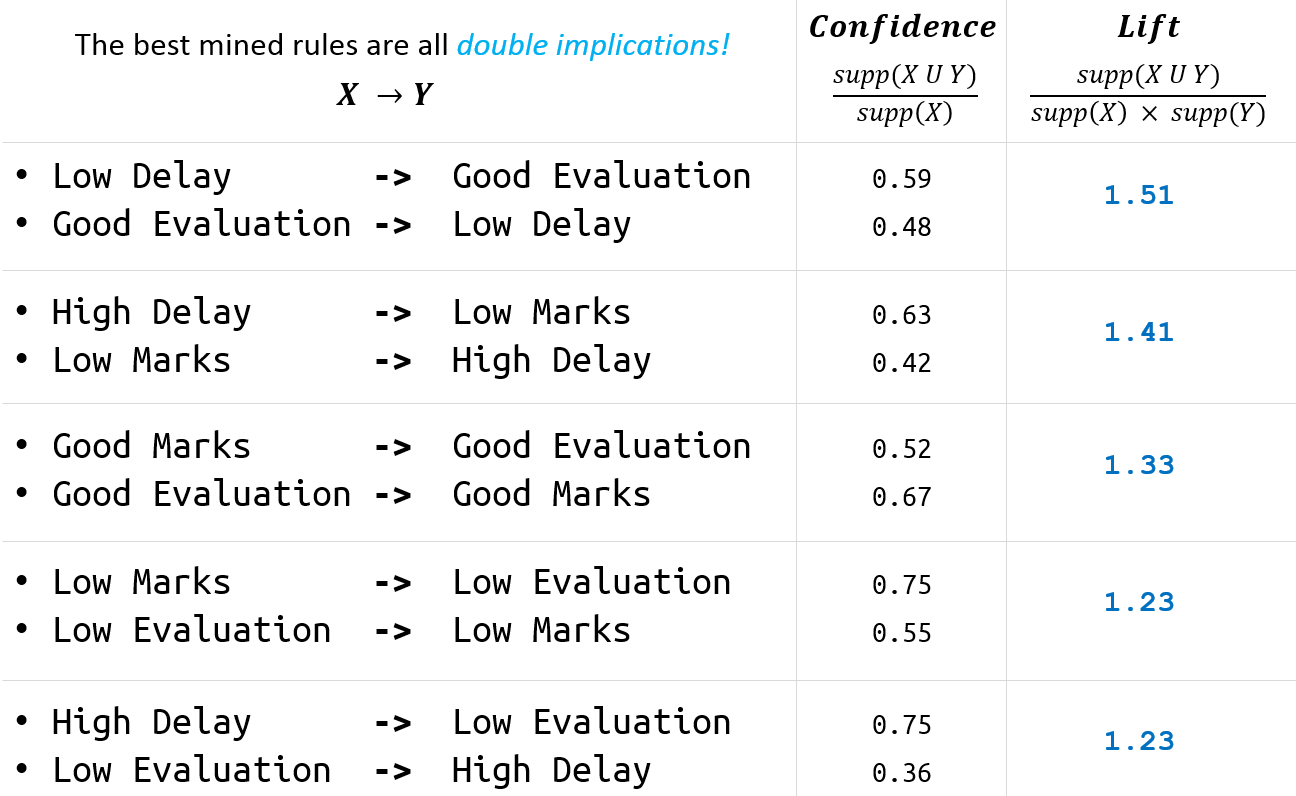
\includegraphics[scale=0.26]{ass6.png}

\end{frame}
